\section{Contiki}
%https://komalbattula.wordpress.com/architecture/
%explain contiki and why we chose it

\subsection{Historic}
\paragraph{}
%https://ieeexplore.ieee.org/stamp/stamp.jsp?tp=&arnumber=1367266
%https://ercim-news.ercim.eu/en76/rd/contiki-bringing-ip-to-sensor-networks
Contiki was created in 2003 by Adam Dunkels. %http://dunkels.com/adam/
At the time, it was the first operating system to provide IP connectivity to sensor networks.
It did so thanks to $\mu$IP, a lightweight TCP/IP stack intended for tiny microcontrollers,
    also developped by Adam Dunkels at the Swedish Institute of Computer Science (now RISE SICS).%https://github.com/adamdunkels/uip

Further developpement of Contiki has been supported by various industries and research institutes 
    such as Texas Instruments, Atmel, Cisco, ENEA, ETH Zurich, Redwire, RWTH Aachen University, 
    Oxford University, SAP, Sensinode, Swedish Institute of Computer Science, ST Microelectronics and Zolertia.
%death?

\subsection{Characteristics and features}
\paragraph{}
The developpement of Contiki started with the need to bring connectivity to small sensor devices with limited capabilities.
By definition, Contiki is not a real-time operating system and has not been designed as such.\\

%memory allocation/stack and kernel/event driven
Contiki operates with the event-driven model.
Processes are implemented as event handlers that run to completion.
An event handler can be defined as a procedure that performs a specific action in response to an event.
Because event handlers cannot block, the same stack can be shared among them.
Also, locking mechanisms are not needed as event handlers do not run concurrently.
Instead of having multiple stacks for multiple threads (which must be over-provisioned or they risk to run out of memory), a single stack can then be used.

This model does not come without problems, as it is sometimes tedious for programmers to manage.
For example, a time-consumming process such as a cryptocraphic operation can monopolize the CPU for quite some time 
    and make the system unable to respond to external events. 
In a preemptive multi-threading system, the computation can be preempted to react to an external event 
    and continue the process later.
To fix this issue, Contiki makes use of an application library that implements preemptible threads.
This library is optional an can be used with programs that explicitly require it.\\

%protothreads
%http://dunkels.com/adam/dunkels05using.pdf
In order to implement its event-driven system, Contiki comes with a mechanism called \textit{protothread}.
The concept of protothreads was also developped by Adam Dunkels with the help of other researchers.
The goal of the protothread programming abstraction is to make it easier for developpers to develop, debug and maintain code written in the event-driven model.

Protothreads can be defined as lightweight stackless threads providing a blocking context on top of an event-driven system.
They can be used to perform non-preemptive concurrency or cooperative multitasking.
Programs written for an event-driven model typically have to be implemented as explicit state machines.
With protothreads, programs can be written in a sequential fashion without designing explicit state machines.

Protothreads do not serve the same purpose as threads for the event-driven model.
The concept has been developped to bring a number of benefits of the multi-threaded programming model into Contiki
    and ease the developpement of applications.\\

%energy saving mechanisms
Contiki does not provide any specific kernel energy saving mechanism.
Instead, it let the application specific parts of the system implement such mechanism.

\subsection{Specificities}
\paragraph{}
%contiki is specific by itself, aims for WSN
%dynamic loading? is that necessary to develop that?
%cooja
Contiki integrates a tool called Cooja.
Cooja is a network simulator which is designed to simulate a network using Contiki motes.
Motes can be simulated at the hardware level or with a standard setup allowing faster response but with less precise system behaviour.
It is an extremely powerful tool which makes developping and debugging tremendously easier even with a large-scale network.

\begin{figure}[!h]
    \centering
    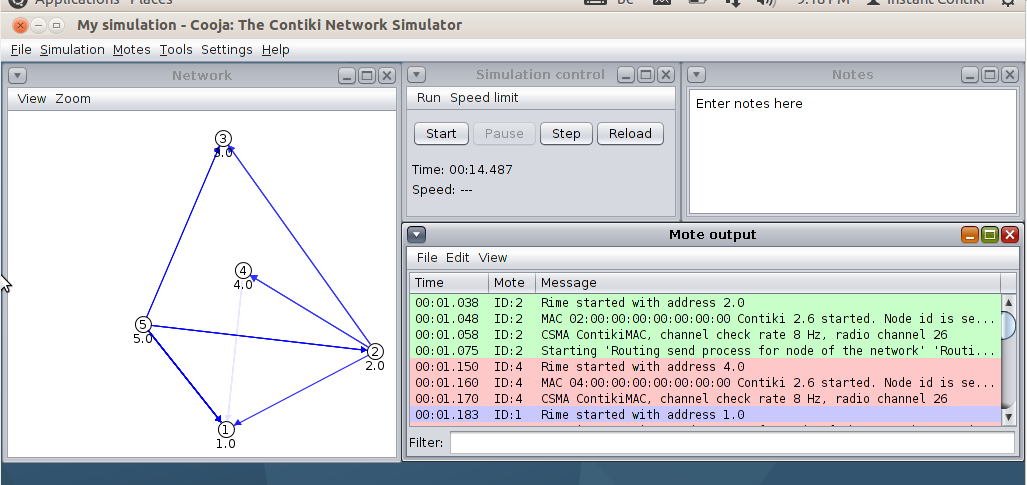
\includegraphics[scale=0.4]{assets/cooja.png}
    \caption{\label{fig:cooja}Cooja interface}
\end{figure}

%rime https://pdfs.semanticscholar.org/9feb/7e0f0d3b507f2f3da60c1b2fea9d5e43449d.pdf
%Contiki provides a low-power radio networking stack called Rime.
%This stack can be used where the full IP stack is not needed.
%The Rime stack can be tuned to 